\documentclass[sigplan]{acmart}
\usepackage[utf8]{inputenc}
\usepackage{amsmath}
\usepackage{amssymb}
\usepackage{amsthm}
\usepackage{bbm}
\usepackage{syntax}
\usepackage{thmtools}
\usepackage{tikz}

\usetikzlibrary{trees}

\title{Finding Singularities via Symbolic Manipulation}
\subtitle{May 1, 2019}

\author{Akash Gaonkar}
\email{akash.gaonkar@colorado.edu}
\affiliation{Undergraduate Student, \institution{University of Colorado at Boulder}}


\author{Valliappan Chidambaram}
\email{vach7169@colorado.edu}
\affiliation{Undergraduate Student, \institution{University of Colorado at Boulder}}

%% Remove footnote with conference information in first column
\renewcommand\footnotetextcopyrightpermission[1]{}
\settopmatter{printacmref=false} % Removes citation information below abstract
\newcommand{\CC}{\ensuremath{\mathbb{C}}}
\newcommand{\ZZ}{\ensuremath{\mathbb{Z}}}
\newcommand{\NN}{\ensuremath{\mathbb{N}}}

\DeclareMathOperator{\sing}{sing}

\let\oldexists\exists
\renewcommand{\exists}{\oldexists\mkern3mu}
\let\oldnexists\nexists
\renewcommand{\nexists}{\oldnexists\mkern3mu}
\let\oldforall\forall
\renewcommand{\forall}{\oldforall\mkern2mu}

\declaretheorem[name=Theorem]{theorem}
\declaretheorem[name=Lemma]{lemma}

\pagestyle{plain}

\theoremstyle{definition}
\declaretheorem[name=Definition]{definition}


\begin{document}

  \begin{abstract}
		Calculus in the complex plane is far more powerful than calculus on the real line. Computers can perform calculus on the real line easily, but it is far more difficult to do so on the complex plane, because much of it relies on the concept of analyticity. For example, by finding singular points, where the function is not analytic, it becomes possible to take integrals over closed loops much easier, and it is easy to know where derivatives exist. We consider a certain class of elementary functions and compositions of these functions. For any such expression, we give an algorithm that attempts to determine where the function has isolated singular points, branch points, and cluster points, and produces its symbolic derivative. We implement this algorithm and evaluate it over several examples, and compare it to existing methods of finding singularities.
  \end{abstract}

  \maketitle

  \section{Introduction}
  \label{sec:introduction}
  A complex function is analytic on some region $R$ if it has a Taylor series that converges to it pointwise on that region. Functions are differentiable on a region $R$ if and only if they are analytic on that region. This means that to take the derivative of a function, you must first know if and where it is analytic. We don't allow expressions that contain functions that are analytic nowhere, like $\overline z$, $Re(z)$, and $Im(z)$, so we only need to find singular points of functions that are mostly analytic. Finding these singular points enables various useful things. For example, if you could classify singular points as isolated, branch, and cluster points, and you could calculate the residues at the isolated singular points, then it would be possible to use the Cauchy-Residue theorem and indented contours to calculate the integral of any closed loop in the complex plane on the allowed functions.

Finding the singular points of a symbolic function is difficult because it is difficult to calculate a Taylor series and test its convergence on a symbolic function. Even if that were possible, it would be difficult to find the singular points, the set of points on which a pointwise convergent Taylor series couldn't be found. It is possible to find the singularities of a function in different ways, using our knowledge of the singularities of simpler expressions, like our method described in Section~\ref{sec:analyticity}. Other computer algebra systems, such as Maple and WolframAlpha use similar methods to calculate singular points in the functions they are given. Maple and WolframAlpha can both find all isolated singular points and branch points of arbitrary functions, although WolframAlpha reports singularities in terms of the inputs to functions (for example, the singularities for $sin(1/z)$ are reported in the $1/z$-plane) and very often fails. Our method allows the user to find all isolated singular points, branch points, and cluster points of functions that we can simplify correctly. When we are unable to solve for the roots of certain equations, we report the answer similar to WolframAlpha. Unlike Maple and WolframAlpha, we are unable to classify our singular points into poles and essential singular points, and we are unable to perform additional computations such as calculating residues at singular points. We are also unable to determine if infinity is a singular point, or the type of singular point at infinity.


  \section{Expressions}
  \label{sec:expressions}
  \begin{figure}[H]
	\setlength{\grammarindent}{5em}
\begin{grammar}
	<Expr> ::= z | \CC\ | sin(<Expr>) | cos(<Expr>) | exp(<Expr>)
	\alt log(<Expr>) | <Sum> | <Term>

	<Sum> ::= <Expr> $\times$ \CC\ | <Expr> $\times$ \CC\ + <Sum>

	<Term> ::= <Expr> \textsuperscript{\CC} | <Expr> \textsuperscript{\CC}  $\times$ <Term>
\end{grammar}

	\caption{The grammar for the allowed expressions}
	\label{fig:grammar}
\end{figure}

Our system allows the expressions defined by \textbf{Expr} in Figure~\ref{fig:grammar}. More specifically, we allow the complex variable $z$, complex numbers, sums, products, powers, sin, cos, log, exp, and compositions of these functions. Each of these expressions are analytic except for a countable number of singular points. The goal of our algorithm is to produce a list of the isolated singular points, branch points, and cluster points. For example, the function $1/log(z-1)$ has an isolated singular point at $z=2$ and a branch point at $z=1$. This is because expressions have isolated singular points where their denominators are $0$, and $log(z-1)=0$ when $z=2$. Expressions also have branch points where the input to a log or non-integer power is zero or infinity, and $z-1=0$ when $z=1$, so that is a branch point. An example with a cluster point would be $1/cos(1/z)$. Its singularities can be found as follows:
\[
	cos\left(\frac{1}{z}\right) = 0
	\implies \frac{1}{z} = \frac{\pi}{2}+n\pi
	\implies z = \frac{1}{\frac{\pi}{2}+n\pi}, \ n\in\ZZ.
\]
Because $lim_{n\to\infty}z=0$, it means that there are an infinite number of singular points about $z=0$, so it's a cluster point. It is also possible for there to be infinitely many cluster points. For example, the singular points of $1/sin(1/sin(z))$ can be found as follows:
\begin{align*}
	& sin\left(\frac{1}{sin(z)}\right) = 0 \implies \frac{1}{sin(z)} = n\pi
	\implies sin(z) = \frac{1}{n\pi} \\
	& \implies z = sin^{-1}\left(\frac{1}{n\pi}\right), \ n\in\ZZ.
\end{align*}
Because $lim_{n\to\infty}z=sin^{-1}(0)=m\pi, \ m \in\ZZ$, there are an infinite number of cluster points. We have shown how to find the singularities of specific expressions, we will now show how to find the singularities for arbitrary expressions.


  \section{Analyticity of Compositions}
  \label{sec:analyticity}
  
We now consider how to systematically find where our expressions are analytic.
Note first that our atoms, $z, \sin, \cos, \log, \cdots$ all have a finite
number of isolated singularities and branch points.

\begin{definition}[Mostly analytic function]
  We say a function is \emph{mostly nonzero, mostly analytic (MNMA)} if it has
  a countable number of zeroes and singularities.
\end{definition}

By definition, our atoms are all MNMA, with the exceptions of the functions
$f(z) = 0, f(z) = \infty$. We now can show that every composition of the other
atoms is MNMA, by noting the following result:

\begin{lemma}[MNMA Compositions are MNMA]
  Compositions of mostly nonzero, mostly analytic functions are mostly
  nonzero, mostly analytic.
\end{lemma}
\begin{proof}
  We proceed by cases. Consider two mostly analytic functions
  $f, g: \CC \to \CC$, with singularities $S_f, S_g \subset \CC$ respectively.
  Also let surjections $m_f: \N \to S_f,\ m_g: \N \to S_g$ count each
  singularity set.
  \begin{description}
    \item[$f + g, f * z$ is mostly analytic.] Consider any point $z$ such that
    both $f$ and $g$ are analytic. Then at such a point, $f(z) + g(z)$ and
    $f(z)g(z)$ must be analytic. Therefore, the singularities of these
    compositions must be a subset of $S_f \cup S_g$.
  \end{description}
\end{proof}

\begin{itemize}
  \item Isolated Singularities -> Rootfinding
  \item Branch Points -> Rootfinding + Singularities
  \item Cluster Points -> Evaluation + Singularities + Branch Points
\end{itemize}


  \section{Symbolic Root Finding}
  \label{sec:rootfinding}
  Our expressions are represented using something known as an abstract syntax tree (AST). ASTs are useful for representing things that can be written as grammars, such as the expressions we allow.
\begin{figure}[H]
	\begin{tikzpicture}[
  tlabel/.style={pos=0.4,right=-1pt,font=\footnotesize\color{red!70!black}},
	level 1/.style={sibling distance=30mm},level 2/.style={sibling distance=20mm}
]
\node{Sum}
child {node {$\times 1$}
	child {node {cos} child {node {z}}}
}
child {node {$\times 1$}
	child {node {exp}
		child {node {Sum}
			child {node {$\times 4i$}
				child {node{z}}
			}
		}
	}
}
child{node {$\times 2$}
	child{node{Term}
		child{node{\textsuperscript{$\wedge$} -2}
			child {node{z}}
		}
		child{node{\textsuperscript{$\wedge$} -1}
			child {node{log} child{node{z}}}
		}
	}
}
;
\end{tikzpicture}

	\caption{Example AST for $cos(z)+e^{4iz}+2/(z^2log(z))$. \\ Note that Sum takes the sum of all of its children, and that Term takes the product of all of its children. Also note that multiplication by a constant takes place in Sums and not Terms. }
	\label{fig:astExample}
\end{figure}
\noindent As you can see in Figure~\ref{fig:astExample}, ASTs can show expressions in a surprisingly intuitive way. To find roots on an AST, the first thing we do is simplify it. We perform simplification on ASTs using rules. These rules say that if a subtree of the AST has some property, then part of it can be replaced with a simplified AST. Some of the rules we use are constant evaluation, removal of things with a coefficient of zero in a Sum, and removal of things with a power of one in a Term. We can't use all of the rules from the real numbers. For example, we allow the simplification $e^{log(z)}\to z$, but not $log(e^z)\to z$, because $log$ is a multivalued function (we could simplify $log(e^z)\to z+2n\pi i$, but this rule was never implemented). We don't have any simplification rules that implement factoring, so we can't successfully simplify the expression $z/(z^2-z)\to 1/(z-1)$, so our algorithms produce incorrect results on such expressions.

We implemented a routine that tried to find where two expressions were equal. To find roots, we ran this routine to find where an expression equaled zero. Our solving routine worked by trying to solve the outermost expression on the right hand side, and calling itself recursively on the input to the outermost expression. For example, when trying to solve $sin(1/z)=0$, we find that $sin(z)=0$ when $z=n\pi$, and then we try to solve $1/z=n\pi$. This doesn't work when trying to solve Sums of more than one expression, or when trying to solve Terms for anything other than zero. We were unable to come up with an algorithm for doing this, so our algorithm simply reports the equations it was unable to solve. WolframAlpha and Maple have similar problems, but they are able to solve more equations with sums and products, and often report numerical solutions when they are unable to solve.


  \section{Results}
  \label{sec:results}
  Our program produced the correct results on everything we tested. Note that we don't keep track of everything in terms of $\pi$s, so they appear as floating point numbers in our solutions.

\begin{figure}[H]
	\raggedright
	Our output: \\
	\begin{verbatim}
Input:    log(-1.000+Z)^-1.000
Deriv:
-1.000*(log(-1.000+Z)^-2.000*(-1.000+Z)^-1.000)
Zeros:    List()
Singular: List(-2.000+Z)
Branch:   List(-1.000+Z)
Cluster:  List()
\end{verbatim} \vspace{7pt}
	WolframAlpha output:\\
	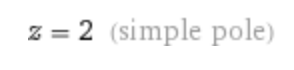
\includegraphics[width=0.4\columnwidth]{images/wpoles1}
	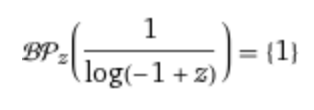
\includegraphics[width=0.4\columnwidth]{images/wbranch1}
	\caption{Our output and WolframAlpha's for $1/log(z-1)$.}
	\label{fig:singEx1}
\end{figure}
Our program outputs zeros, singular points, branch points, and cluster points in terms of equations that should equal zero. This means that our program found a singular point at $z=2$ and a branch point at $z=1$, which is the same as the results from when we did it manually in Section~\ref{sec:expressions}, and the same as WolframAlpha's results.

\begin{figure}[H]
	\raggedright
	Our output: \\
	\begin{verbatim}
Input:    cos(Z^-1.000)^-1.000
Deriv:    -1*(cos(Z^-1)^-2*Z^-2*sin(Z^-1))
Zeros:    List()
Singular:
List(-1*((1.571+3.142*n1)^-1*(e^(-6.283i*n2)))+Z)
Branch:   List()
Cluster:  List(Z)
	\end{verbatim} \vspace{7pt}
	WolframAlpha output:\\
	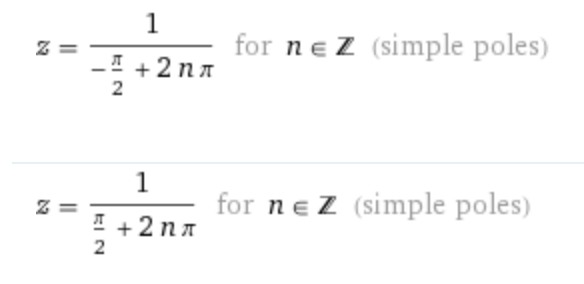
\includegraphics[width=0.6\columnwidth]{images/wpoles2}
	\caption{Our output and WolframAlpha's for $1/cos(1/z)$, some decimals have been truncated for brevity.}
	\label{fig:singEx2}
\end{figure}
While it may not be obvious from the start, our output, WolframAlpha's, and what we worked out in Section~\ref{sec:expressions} are equivalent, with the exception that WolframAlpha doesn't report cluster points. The $e^{-6.283in_2}$ exists because we don't have a rule to simplify it to $1$.

\begin{figure}[H]
	\raggedright
	Our output: \\
	\begin{verbatim}
Input:    sin(sin(Z)^-1.000)^-1.000
Deriv:
sin(sin(Z)^-1)^-2*sin(Z)^-2*cos(sin(Z)^-1)*cos(Z)
Zeros:    List()
Singular:
List(-1*asin(0.318*((e^(-6.283i*n2))*n1^-1))+
-6.283*n3+Z)
Branch:   List()
Cluster:  List(-3.142*n5+-6.283*n3+Z)
	\end{verbatim} \vspace{7pt}
	WolframAlpha output:\\
	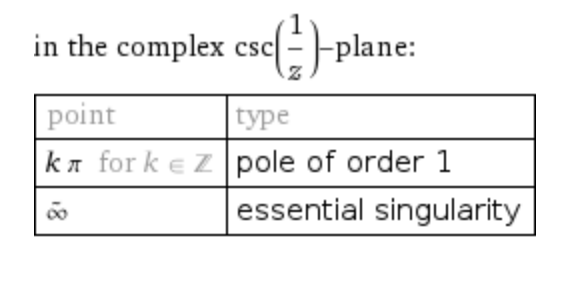
\includegraphics[width=0.6\columnwidth]{images/wpoles3}
	\caption{Our output and WolframAlpha's for $1/sin(1/sin(z))$, some decimals have been truncated for brevity. Note that $1/\pi=0.318.$}
	\label{fig:singEx3}
\end{figure}
Our output is once again equivalent to what we derived in Section~\ref{sec:expressions}, with the exception that there are many more quantifiers (the $n_i$'s), that haven't been simplified out. WolframAlpha technically outputs the same thing, but it fails to solve the equations and instead outputs the answer in terms of the $csc(1/z)$-plane, which makes its results harder to interpret and use. It also doesn't identify cluster points.


  \section{Conclusion and Future Work}
  \label{sec:conclusion}
  We have shown that our method is not only able to find and detect isolated singular points and branch points, but also cluster points, which WolframAlpha doesn't do. Furthermore, our method solves certain cases of singularities that WolframAlpha doesn't, like $1/sin(1/sin(z))$. We aren't able to solve some cases that WolframAlpha can, like $1/f(z)$ where f is a polynomial, but this would be easily fixed with future work. We also don't classify isolated singular points into poles and essential singularities, but this could also be solved with future work. Our algorithm is easily extensible, and it is possible for us to achieve performance much better than WolframAlpha's singularity finding.

There are many improvements that can be made to our algorithm and its implementation. The main issue with our current algorithm is our inability to completely simplify expressions, because this leads to incorrect answers on inputs like $z/(z^2-z)$. These kinds of problems could be mostly solved by introducing factoring and expanding into our simplify function, which would allow us to cancel common terms, like the $z$ in the earlier expression. Another change we could make to our simplification algorithm would be to allow branching. Currently, the algorithm greedily applies whatever rules match the current expression, but it might simplify something that would remove the possibility of other simplification steps, which is suboptimal. Branching would allow us to try more possibilities and get more simplified expressions. We could also simply add more rules. The next problem in our algorithm is our inability to solve most equalities consisting of Sums and Terms. We would be able to solve this to some extent by figuring out a way to factor/expand some expressions to produce compositions of polynomials and other functions, which we could then attempt to solve. However, polynomials of degree 5 and above wouldn't be solvable without numerical techniques. Some expressions, like $z+sin(z)$, couldn't be simplified into polynomials, so we would also need numerical root-finding for these expressions. This still wouldn't work if an expression in the equality contained quantifiers. While solving the problem in general is impossible, even for WolframAlpha and Maple, these techniques would greatly increase the number of functions our algorithm would be able to provide answers for. The other big problems in our system are our inability to simplify subexpressions containing quantifiers, and the fact that we use floating point numbers instead of $\pi$ and $e$. Quantifier simplification is an extremely hard problem because quantifiers are elements of \ZZ. An example of this difficulty is $c_1n_1+c_2n_2$, where $Re(c_1)/Re(c_2)$ or $Im(c_1)/Im(c_2)$ is irrational, because this would simplify to some subset of \CC, and it would likely be difficult or impossible to represent this subset in terms of quantifiers. The problem of $\pi$ and $e$, is solvable by introducing new elements into the AST, and changing how constant expressions are evaluated, but this would take lots of time to implement correctly.


All code in our project is available on: \\ \href{https://github.com/Anonymous-Stranger/complex-differentiation/tree/expr-rewrite}{https://github.com/Anonymous-Stranger/complex-differentiation/tree/expr-rewrite}


  \nocite{*}
  \bibliographystyle{acm}
  \bibliography{sources}

\end{document}
